%!TEX program = xelatex
%!TEX TS-program = xelatex
%!TEX encoding = UTF-8 Unicode

\documentclass[aspectratio=169]{beamer}
\usepackage[UTF8, heading = false, scheme = plain]{ctex}
\usepackage{silence}
\WarningFilter{biblatex}{Patching footnotes failed}
\usepackage[hyperref=true,backend=biber,sorting=none,backref=true,style=ieee]{biblatex}
\addbibresource{references.bib}
\renewcommand{\footnotesize}{\tiny}
\usepackage{graphicx}
\usepackage{subfig}
\usepackage{caption}
\captionsetup{font={scriptsize}}
\renewcommand\figurename{图}
\newcommand\blfootnote[1]{%
  \begingroup
  \renewcommand\thefootnote{}\footnote{#1}%
  \addtocounter{footnote}{-1}%
  \endgroup
}
% \usepackage{tikz}

% \usetheme{Madrid}
% \titlegraphic{
\includegraphics[width=2cm, height=2cm]{fig/jnulogo.png}}
\title{Private Aggregation of Teacher Ensembles}
\subtitle{用半监督知识迁移解决深度学习中训练数据隐私问题}
% \author{
\includegraphics[width=2cm, height=2cm]{fig/jnulogo.png}}
\author{熊凯亚}
\date{\today}
\institute[JNU]{Jinan University}

\begin{document}
\begin{frame}
\titlepage
\end{frame}

\begin{frame}{Outline}
\tableofcontents[
    currentsection,
    sectionstyle=show,
    subsectionstyle=show
  ]
\end{frame}

\section{PATE}
\begin{frame}{PATE}
Google在ICLR'17上发表的文章\cite{Papernot2016SemisupervisedKT}\footfullcite{Papernot2016SemisupervisedKT}用半监督知识迁移解决深度学习中训练数据隐私问题,为了解决这个问题这篇文章提出了PATE(Private Aggregation of Teacher Ensembles)教师全体的隐私聚合的概念。
\end{frame}

\subsection{背景}
\begin{frame}{背景}
对于训练一般人脸识别模型例子:
\begin{enumerate}
\item 2015年的一项研究发现\footfullcite{fredrikson2015model},通过模型的预测结果,可以反过来重建模型训练时使用的人脸数据(model inversion attacks)。
\item 2016年另一项研究发现\footfullcite{shokri2017membership},同样可以根据模型的预测结果,来推理出模型训练数据中是否包含了某个具体的训练点(training point),这种攻击称为会员推理攻击(membership inference attacks)。
\end{enumerate}
\end{frame}

\subsection{威胁模型}
\begin{frame}{威胁模型}
两种攻击类型:
\begin{enumerate}
\item model querying,模型查询:黑盒攻击,攻击者通过查询来观察模型。对于攻击者而言模型是一个黑盒,攻击者可以挑选输入值来观察模型的预测结果。
\item model inspection,模型检验:属于白盒攻击。攻击者知道模型的结构和参数,例如\cite{hitaj2017deep}\footfullcite{hitaj2017deep}协作学习中的参与者对模型进行的白盒攻击。
\end{enumerate}
攻击假设:
\begin{itemize}
\item 攻击者可以进行潜在的无限多次的查询(黑盒)。
\item 攻击者能够进入到模型的内部组件(白盒)。
\end{itemize}
\end{frame}

\subsection{教师模型}
\begin{frame}{教师模型}
Approach:在不相交的子集上训练教师模型,然后在使用另外的未标记的非敏感数据对学生模型进行训练。
\begin{enumerate}
\item 将待训练的敏感数据分为互斥的$N$份不同数据集,分别独立训练不同的模型,得到$N$个教师模型。
\item 部署训练好的教师模型时,需要记录每一个教师模型对于查询的预测结果,选取票数最高的那个预测结果,并将预测结果聚合起来。
\item 在统计票数之后引入拉普拉斯噪声,将票数的统计情况打乱(票数会泄露隐私),从而保护了隐私。
\end{enumerate}

教师模型的训练及聚集过程如图\ref*{fig:teacher-model}所示。
\end{frame}

\begin{frame}{教师模型}
\begin{figure}[!h]
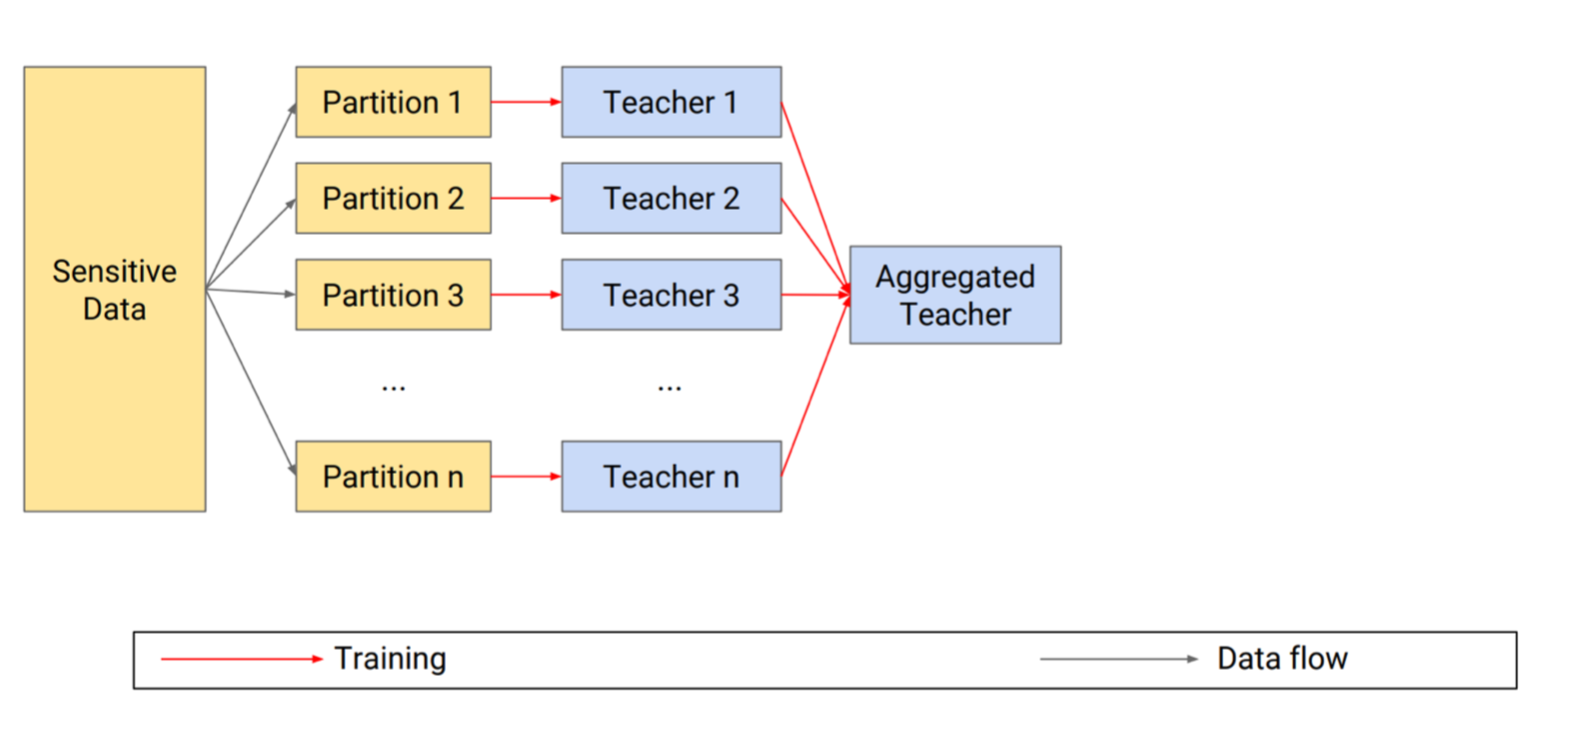
\includegraphics[width = \linewidth]{fig/teacher-model.png}
\caption{教师模型的聚集过程}
\label{fig:teacher-model}
\end{figure}
\end{frame}

\begin{frame}{教师模型}
\begin{figure}[!h]
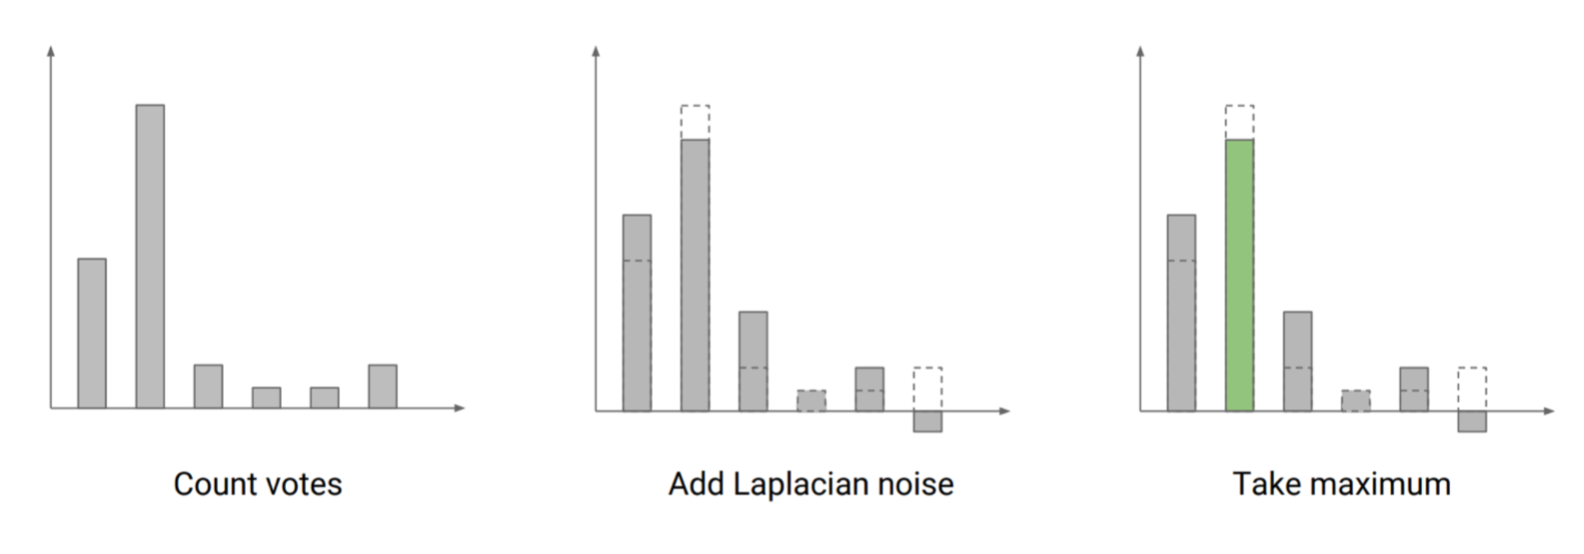
\includegraphics[width = \linewidth]{fig/aggergation.png}
\label{fig:aggergation}
\end{figure}
\begin{itemize}
\item 如果大部分教师模型都同意某一个预测结果,即不依赖于具体的分散数据集,隐私成本很小。
\item 如果有两类预测结果有相近的票数,那么这种不一致,或许会泄露隐私信息。
\end{itemize}
\end{frame}

\subsection{学生模型}
\begin{frame}{学生模型}
\begin{itemize}
\item 聚合教师模型可以看作是一个差分隐私API,用户提交输入值,模型就会返回相应的标签,同时又能保护隐私。
\item 但是,如果训练一个模型,部署到用户设备上直接运行模型得出预测结果,这样的话肯定会更好。为了训练学生模型,需要聚合教师模型以隐私保护的方式,来给公共数据进行标注,传递知识。
\end{itemize}
\end{frame}

\begin{frame}{学生模型}
\begin{figure}[!h]
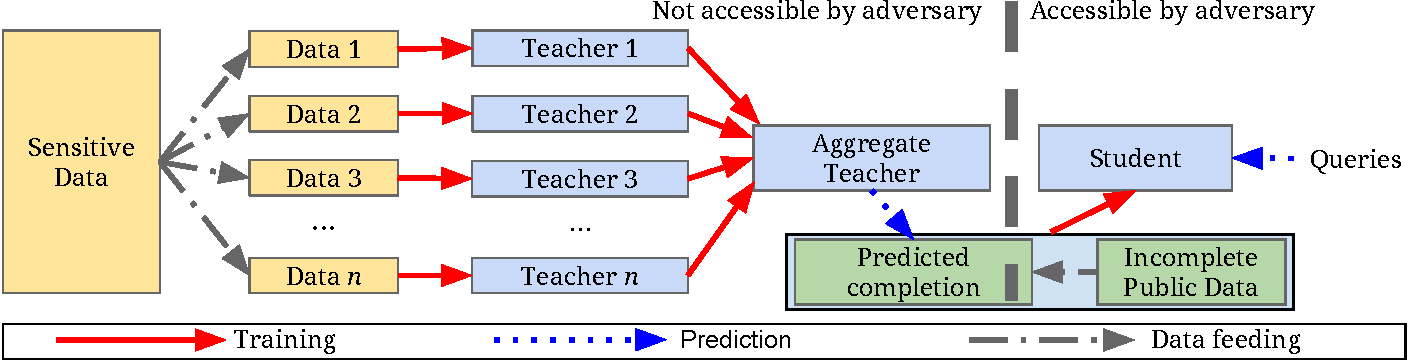
\includegraphics[width = \linewidth]{fig/approach-overview.pdf}
\caption{学生模型的训练}
\label{fig:overview}
\end{figure}
使用未标记的公开数据训练学生模型,部分数据使用对教师模型的查询结果进行标记。
\end{frame}

\begin{frame}{学生模型}
学生模型的必要性:
\begin{enumerate}
\item 每次查询聚合教师模型,都会增加隐私成本。训练学生模型后,只能对聚合教师模型进行固定数量的查询,隐私成本就会被固定下来。
\item 需要防范攻击者探取模型底层函数库。教师模型是由隐私数据训练的,学生模型是由公共数据(非隐私数据)训练的,带有隐私保护的标注。即使攻击者获取到学生模型的训练数据,也只能得到带有隐私保护的标签信息。
\end{enumerate}
总体上:
\begin{itemize}
\item 教师模型用来防御白盒攻击
\item 学生模型用来防御黑盒攻击
\end{itemize}
\end{frame}

\section{PATE-G}
\begin{frame}{PATE-G}
\begin{figure}[!h]
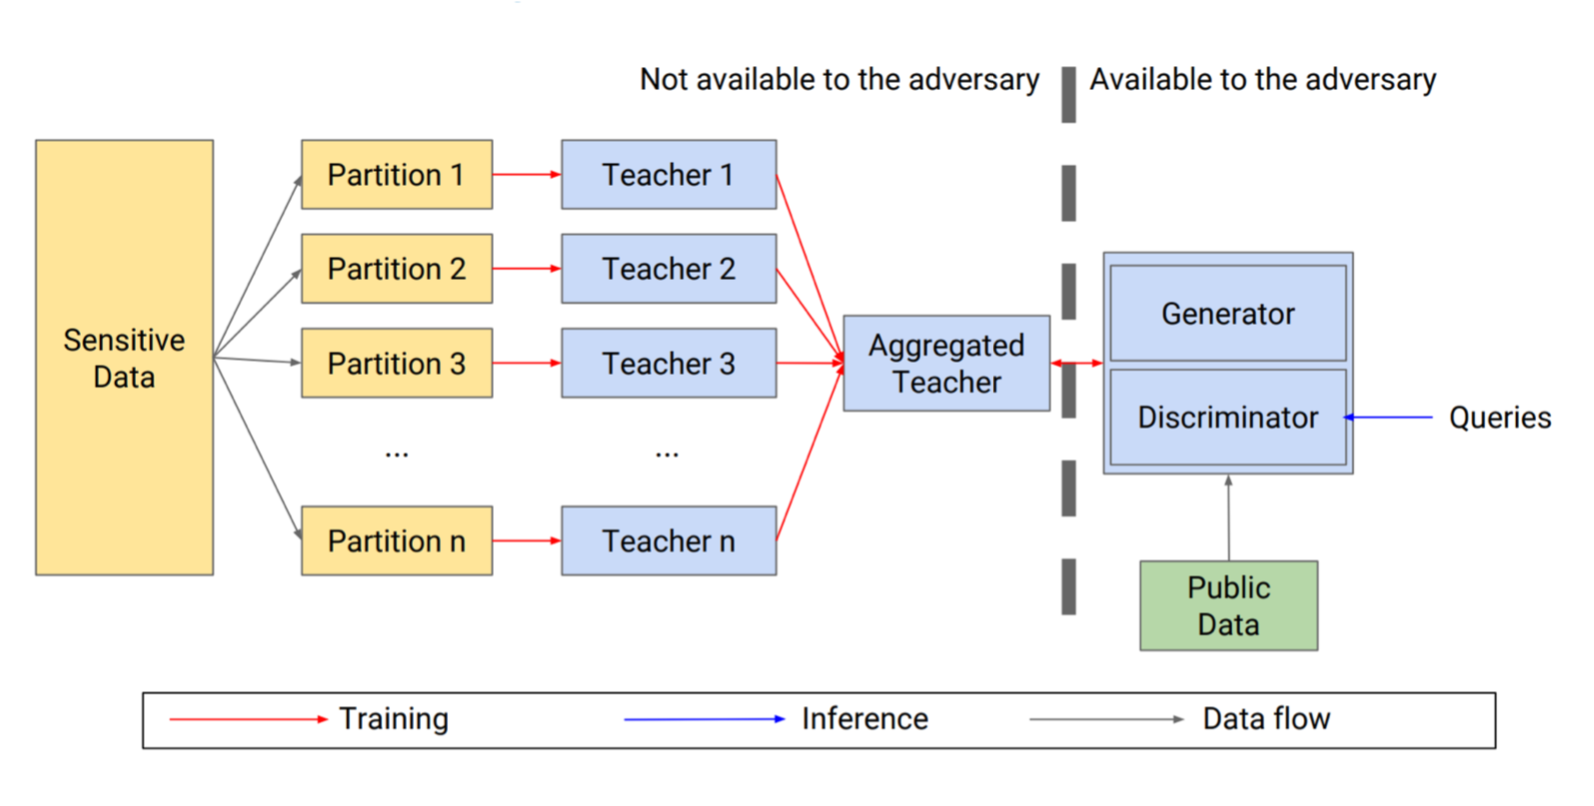
\includegraphics[width = 4in]{fig/student-model-gan.png}
\caption{使用GAN训练学生模型}
\end{figure}
\begin{itemize}
\item 将原本二元分类的判别器扩展至一个多类别的分类器,区分:已标注的真实样本,未标注真实样本,以及生成样本。
\item 训练之后只使用判别器来处理查询。
\end{itemize}
\end{frame}

\section{实验}
\begin{frame}{实验}
使用了四个数据集:MNIST、SVHN、UCI Adult 和 UCI Diabetes。如图所示:
\begin{figure}
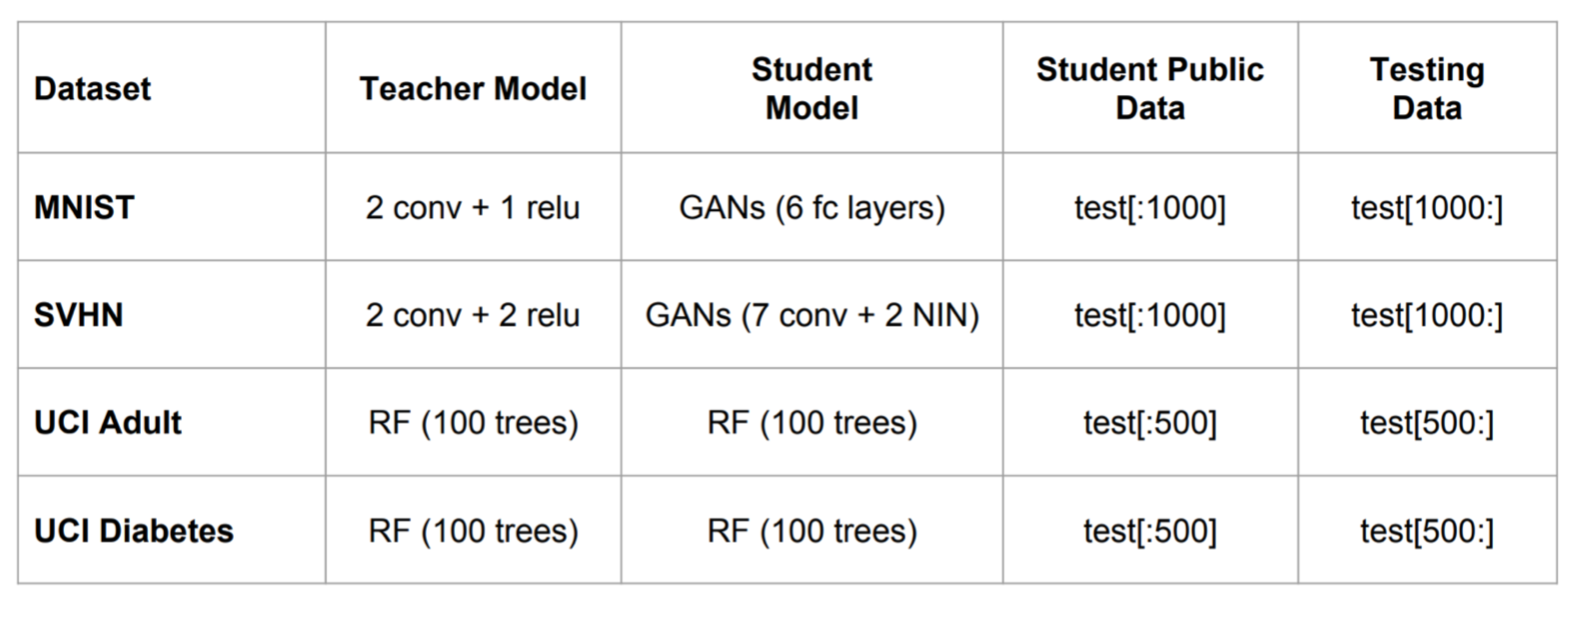
\includegraphics[width = \linewidth]{fig/experiment-settings.png}
\caption{实验数据集}
\end{figure}
\end{frame}

\subsection{教师模型准确率}
\begin{frame}{教师模型准确率}
图\ref{fig:teacher-accuracy}描绘了聚合教师模型的准确率。在训练学生模型之前,需要考虑了每一个标签的隐私。横轴是每一个标签查询的$\epsilon$值,纵轴是预测结果的平均准确率。
\begin{figure}
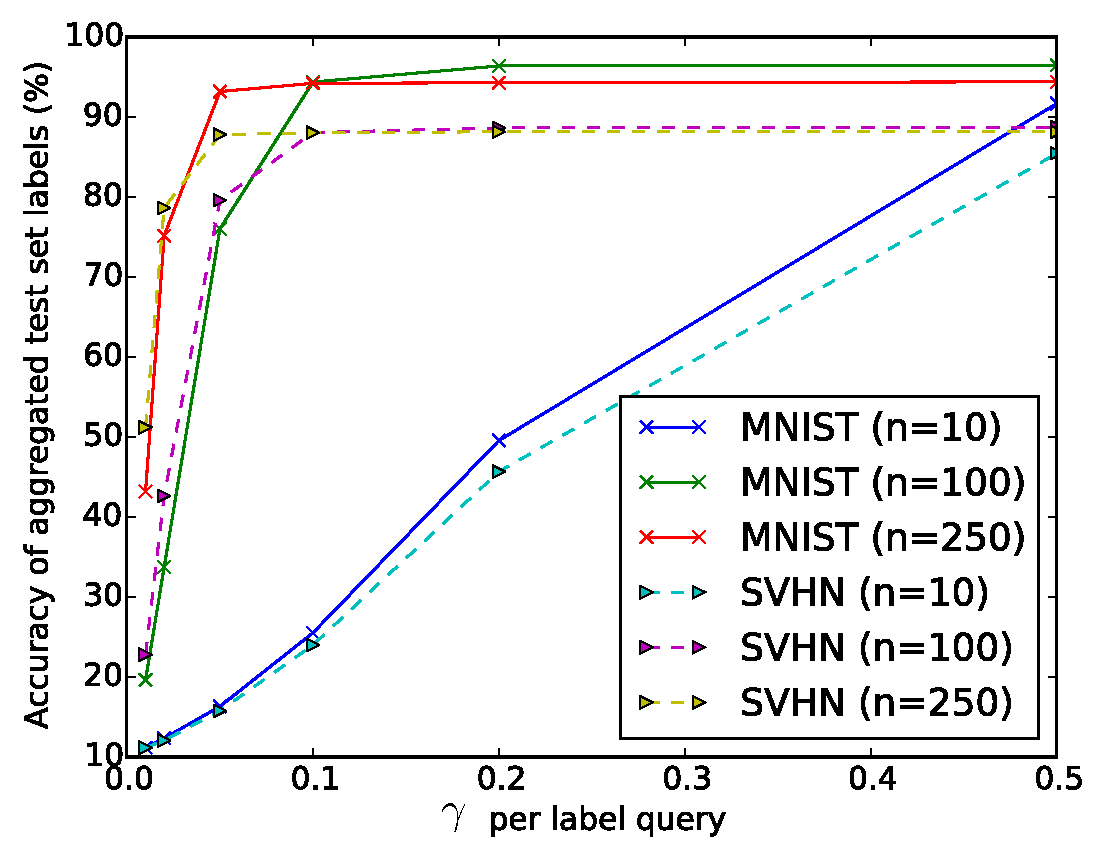
\includegraphics[width = 2.3in]{fig/lap-scale-accuracy.pdf}
\caption{聚合教师模型准确率}
\label{fig:teacher-accuracy}
\end{figure}
\blfootnote{
紫色的线代表10个聚合教师模型($n=10$)。逐渐降低$\epsilon$值,准确率也很快下降。但如图中绿线和红线的部分,分别包含100个和250个聚合教师模型($n=100, n=250$),在较低$\epsilon$值时,仍可以保持较高的准确率。}
\end{frame}

\subsection{对比}
\begin{frame}{对比}

\begin{figure}
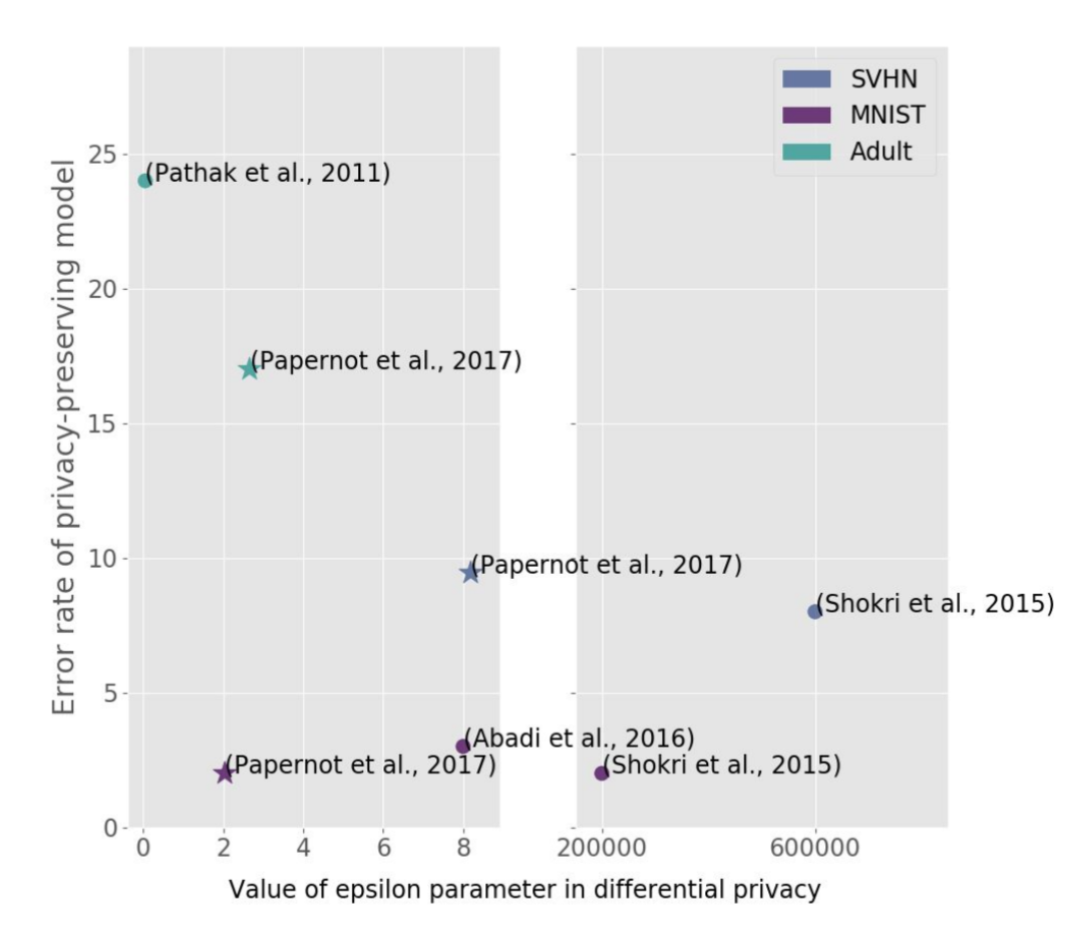
\includegraphics[width = 2.1in]{fig/approach-comparison.png}
\caption{不同Approach的对比}
\end{figure}
\blfootnote{Papernot, M. Abadi, Ú. Erlingsson, et al., “Semi-supervised knowledge transfer for deep learning from private training data,” CoRR,
vol. abs/1610.05755, 2016.}
\blfootnote{Abadi, A. Chu, I. Goodfellow, et al., “Deep learning with differential privacy,” in Proceedings of the 2016 ACM SIGSAC Conference on
Computer and Communications Security, ACM, 2016, pp. 308–318.}
\blfootnote{Shokri and V. Shmatikov, “Privacy-preserving deep learning,” in Proceedings of the 22nd ACM SIGSAC conference on computer and
communications security, ACM, 2015, pp. 1310–1321.}
\end{frame}

% \section{总结}
% \begin{frame}{总结}
% \begin{enumerate}
% \item 这个方法是具有通用性,不依赖于特定的学习算法可以将它应用于各种分类器中(包括神经网络)。
% \item 差分隐私范围(bound)不是给定的,对于达到准确度与隐私之间的良好的平衡,具有重要意义。
% \item 隐私性和通用性并不一定是互相矛盾的。
% \end{enumerate}
% \end{frame}

\begin{frame}{References}
\printbibliography
\end{frame}
\end{document}
